% ============================================================
%  PRÉSENTATION BEAMER — Projet PF22 — Approche Multi-Fidélité
%  Auteur : Ivann Vasic — UTBM — Mars–Juin 2026
%  Version : refonte stylistique professionnelle
% ============================================================
\documentclass[aspectratio=169, 10pt]{beamer}

% ============================================================
%  PAQUETS
% ============================================================
\usepackage[utf8]{inputenc}
\usepackage[T1]{fontenc}
\usepackage[french]{babel}
\usepackage{lmodern}
\usepackage{helvet}
\renewcommand{\familydefault}{\sfdefault}
\usepackage{microtype}
\usepackage{graphicx}
\usepackage{booktabs}
\usepackage{tabularx}
\usepackage{multirow}
\usepackage{array}
\usepackage{colortbl}
\usepackage{tikz}
\usetikzlibrary{shapes.geometric, arrows.meta, positioning, fit, backgrounds, calc, shadows.blur}
\usepackage{xcolor}
\usepackage{pgfplots}
\pgfplotsset{compat=1.18}
\usepackage{amsmath}
\usepackage{amssymb}
\usepackage{fontawesome5}

% ============================================================
%  PALETTE — bleu nuit, sarcelle, ambre (éditoriale, sobre)
% ============================================================
\definecolor{primary}{RGB}{18,36,66}          % bleu nuit profond
\definecolor{primarydk}{RGB}{10,22,44}        % encore plus sombre
\definecolor{accent}{RGB}{14,165,164}         % sarcelle moderne
\definecolor{accentlight}{RGB}{186,230,228}   % sarcelle clair
\definecolor{gold}{RGB}{217,164,65}           % ambre / or doux
\definecolor{goldlight}{RGB}{246,228,192}
\definecolor{paper}{RGB}{248,249,251}         % fond papier
\definecolor{card}{RGB}{255,255,255}          % cartes blanches
\definecolor{rule}{RGB}{222,227,235}          % lignes fines
\definecolor{ink}{RGB}{28,36,52}              % texte principal
\definecolor{muted}{RGB}{110,122,142}         % texte secondaire
\definecolor{hfcolor}{RGB}{31,81,140}         % HF : bleu profond
\definecolor{bfcolor}{RGB}{142,152,170}       % BF : gris-bleu
\definecolor{success}{RGB}{46,139,87}         % vert sobre
\definecolor{warn}{RGB}{205,133,63}
\definecolor{danger}{RGB}{176,58,58}

% ============================================================
%  THÈME BEAMER PERSONNALISÉ
% ============================================================
\usetheme{default}
\usecolortheme{default}
\setbeamertemplate{navigation symbols}{}
\setbeamertemplate{frametitle continuation}{}

\setbeamercolor{background canvas}{bg=paper}
\setbeamercolor{normal text}{fg=ink}
\setbeamercolor{frametitle}{fg=primary, bg=paper}
\setbeamerfont{frametitle}{series=\bfseries, size=\large}
\setbeamercolor{title}{fg=white}
\setbeamercolor{subtitle}{fg=accentlight}
\setbeamercolor{author}{fg=accentlight}
\setbeamercolor{date}{fg=muted}
\setbeamercolor{item}{fg=accent}
\setbeamercolor{subitem}{fg=muted}
\setbeamertemplate{itemize item}{\color{accent}\small\faAngleRight}
\setbeamertemplate{itemize subitem}{\color{muted}\scriptsize$\blacktriangleright$}
\setbeamerfont{block title}{series=\bfseries, size=\small}

% ------------------------------------------------------------
%  Footer sobre : filet fin + mentions discrètes
% ------------------------------------------------------------
\setbeamertemplate{footline}{%
  \begin{beamercolorbox}[wd=\paperwidth, ht=0.5cm, dp=0.25cm]{footline}%
    \begin{tikzpicture}[overlay, remember picture]
      \draw[rule, line width=0.4pt]
        ([xshift=0.7cm, yshift=0.72cm]current page.south west) --
        ([xshift=-0.7cm, yshift=0.72cm]current page.south east);
      \node[anchor=west, text=muted, font=\scriptsize]
        at ([xshift=0.7cm, yshift=0.38cm]current page.south west)
        {Ivann Vasic\,\textbf{\textbar}\,Projet PF22\,\textbf{\textbar}\,UTBM 2026};
      \node[anchor=east, text=muted, font=\scriptsize]
        at ([xshift=-2.4cm, yshift=0.38cm]current page.south east)
        {R\'{e}duction des co\^{u}ts d'apprentissage};
      \node[anchor=east, text=primary, font=\scriptsize\bfseries]
        at ([xshift=-0.7cm, yshift=0.38cm]current page.south east)
        {\insertframenumber\,/\,\inserttotalframenumber};
    \end{tikzpicture}%
  \end{beamercolorbox}%
}

% ------------------------------------------------------------
%  Frametitle : accent sarcelle + filet + sous-titre à droite
% ------------------------------------------------------------
\setbeamertemplate{frametitle}{%
  \nointerlineskip%
  \vspace{0.25cm}%
  \begin{beamercolorbox}[wd=\paperwidth, ht=0.85cm, dp=0.1cm, leftskip=0.8cm, rightskip=0.8cm]{frametitle}%
    \begin{tikzpicture}[overlay]
      \fill[accent] (-0.45cm, -0.05cm) rectangle (-0.15cm, 0.62cm);
    \end{tikzpicture}%
    {\usebeamerfont{frametitle}\color{primary}\insertframetitle}%
    \ifx\insertframesubtitle\empty\else
      \hfill{\color{muted}\footnotesize\textit{\insertframesubtitle}}%
    \fi\\[-0.1em]
    \textcolor{rule}{\rule{\dimexpr\paperwidth-1.6cm\relax}{0.4pt}}%
  \end{beamercolorbox}%
  \vspace{0.1cm}%
}

% ------------------------------------------------------------
%  Blocks — trois variantes sobres
% ------------------------------------------------------------
\setbeamercolor{block title}{bg=primary, fg=white}
\setbeamercolor{block body}{bg=card, fg=ink}
\setbeamercolor{block title alerted}{bg=danger, fg=white}
\setbeamercolor{block body alerted}{bg=danger!6, fg=ink}
\setbeamercolor{block title example}{bg=success, fg=white}
\setbeamercolor{block body example}{bg=success!7, fg=ink}

% ============================================================
%  MÉTADONNÉES
% ============================================================
\title{\textbf{R\'{e}duction des Co\^{u}ts d'Apprentissage}}
\subtitle{par Approche Multi-Fid\'{e}lit\'{e}}
\author{Ivann Vasic}
\institute{UTBM --- Universit\'{e} de Technologie de Belfort-Montb\'{e}liard}
\date{Pr\'{e}sentation de mi-parcours --- Mars--Juin 2026}

% ============================================================
%  COMMANDES UTILITAIRES
% ============================================================
\newcolumntype{L}[1]{>{\raggedright\arraybackslash}p{#1}}
\newcolumntype{C}[1]{>{\centering\arraybackslash}p{#1}}

% Carte générique (fond blanc, ombre douce)
\newcommand{\card}[2][card]{%
  \tikz[baseline=(x.base)]{\node[fill=#1, rounded corners=2pt, inner sep=4pt,
    drop shadow={shadow xshift=0pt, shadow yshift=-0.4pt, opacity=0.08}] (x) {#2};}%
}

% KPI (grand chiffre + label)
\newcommand{\kpi}[3]{%
  \begin{tikzpicture}
    \node[fill=card, rounded corners=3pt, draw=rule, line width=0.4pt,
          minimum width=3.1cm, minimum height=1.55cm, inner sep=5pt] (k) {};
    \node[anchor=north] at ([yshift=-0.1cm]k.north) {\textcolor{#1}{\Large\bfseries #2}};
    \node[anchor=south, text=muted, font=\scriptsize, text width=2.9cm, align=center]
      at ([yshift=0.1cm]k.south) {#3};
  \end{tikzpicture}%
}

% ============================================================
\begin{document}
% ============================================================

% ============================================================
%  SLIDE DE TITRE
% ============================================================
{
\setbeamertemplate{footline}{}
\setbeamertemplate{frametitle}{}
\begin{frame}[plain]
  \begin{tikzpicture}[overlay, remember picture]
    % Fond dégradé simulé (deux rectangles superposés)
    \fill[primarydk] (current page.south west) rectangle (current page.north east);
    \shade[top color=primary, bottom color=primarydk]
      (current page.south west) rectangle (current page.north east);

    % Motif géométrique discret (cercles)
    \fill[accent, opacity=0.10] ([xshift=-3cm, yshift=-1cm]current page.north east) circle (5.5cm);
    \fill[accent, opacity=0.15] ([xshift=-1.5cm, yshift=-2cm]current page.north east) circle (3cm);
    \fill[gold, opacity=0.18] ([xshift=-0.5cm, yshift=-1cm]current page.north east) circle (1.2cm);

    % Bande latérale d'accent
    \fill[accent] (current page.south west) rectangle ([xshift=0.18cm]current page.north west);

    % En-tête institutionnel
    \node[anchor=north west, text=accentlight, font=\footnotesize\bfseries, text width=10cm]
      at ([xshift=0.95cm, yshift=-0.7cm]current page.north west)
      {UNIVERSIT\'{E} DE TECHNOLOGIE DE BELFORT-MONTB\'{E}LIARD};
    \node[anchor=north west, text=muted, font=\scriptsize]
      at ([xshift=0.95cm, yshift=-1.15cm]current page.north west)
      {PROJET PF22\quad\textbullet\quad D\'{E}PARTEMENT INFORMATIQUE};

    % Filet fin de séparation
    \draw[accent, line width=0.8pt]
      ([xshift=0.95cm, yshift=-1.55cm]current page.north west) --
      ([xshift=2.5cm, yshift=-1.55cm]current page.north west);

    % Titre principal (gros, étagé)
    \node[anchor=north west, text=white, font=\fontsize{24}{28}\bfseries\selectfont, text width=11cm]
      at ([xshift=0.95cm, yshift=-2cm]current page.north west)
      {R\'{e}duction des Co\^{u}ts};
    \node[anchor=north west, text=white, font=\fontsize{24}{28}\bfseries\selectfont, text width=11cm]
      at ([xshift=0.95cm, yshift=-2.95cm]current page.north west)
      {d'Apprentissage};
    \node[anchor=north west, text=accent, font=\Large\bfseries, text width=11cm]
      at ([xshift=0.95cm, yshift=-3.95cm]current page.north west)
      {par Approche Multi-Fid\'{e}lit\'{e}};

    % Baseline descriptive
    \node[anchor=north west, text=accentlight!85, font=\small, text width=10cm]
      at ([xshift=0.95cm, yshift=-4.85cm]current page.north west)
      {Exploration de la combinaison de donn\'{e}es Haute et Basse Fid\'{e}lit\'{e} pour r\'{e}duire le co\^{u}t d'acquisition des jeux de donn\'{e}es en deep learning.};

    % Séparateur bas
    \draw[accent, line width=0.6pt]
      ([xshift=0.95cm,  yshift=1.85cm]current page.south west) --
      ([xshift=6cm, yshift=1.85cm]current page.south west);

    % Signature auteur
    \node[anchor=west, text=white, font=\normalsize\bfseries]
      at ([xshift=0.95cm, yshift=1.4cm]current page.south west)
      {Ivann Vasic};
    \node[anchor=west, text=accentlight, font=\footnotesize]
      at ([xshift=0.95cm, yshift=0.95cm]current page.south west)
      {\'{E}tudiant Ing\'{e}nieur --- UTBM};
    \node[anchor=west, text=muted, font=\scriptsize]
      at ([xshift=0.95cm, yshift=0.45cm]current page.south west)
      {Mars -- Juin 2026\quad\textbullet\quad Pr\'{e}sentation de mi-parcours};
  \end{tikzpicture}
\end{frame}
}

% ============================================================
%  SLIDE PLAN
% ============================================================
{
\setbeamertemplate{footline}{}
\begin{frame}[plain]
  \begin{tikzpicture}[overlay, remember picture]
    \shade[top color=primary, bottom color=primarydk]
      (current page.south west) rectangle (current page.north east);
    \fill[accent] (current page.south west) rectangle ([xshift=0.18cm]current page.north west);

    \node[anchor=north west, text=accent, font=\footnotesize\bfseries]
      at ([xshift=0.95cm, yshift=-0.7cm]current page.north west)
      {SOMMAIRE};
    \node[anchor=north west, text=white, font=\LARGE\bfseries]
      at ([xshift=0.95cm, yshift=-1.15cm]current page.north west)
      {Plan de la pr\'{e}sentation};
    \draw[accent, line width=0.8pt]
      ([xshift=0.95cm, yshift=-2.05cm]current page.north west) --
      ([xshift=2.5cm, yshift=-2.05cm]current page.north west);
  \end{tikzpicture}

  \vspace{2.1cm}
  \begin{columns}[T]
    \begin{column}{0.47\textwidth}
      \begin{tikzpicture}
        \foreach \n/\t in {
          1/{Contexte et objectifs},
          2/{Environnement de travail},
          3/{Jeu de donn\'{e}es \& pipeline},
          4/{Architecture ResNet-18}
        } {
          \pgfmathsetmacro{\y}{-(\n-1)*0.95}
          \fill[white, opacity=0.05, rounded corners=3pt] (0, \y) rectangle (7.0, \y+0.72);
          \draw[accent, line width=0.8pt] (0, \y+0.05) -- (0, \y+0.67);
          \node[anchor=west, text=accent, font=\small\bfseries]
            at (0.25, \y+0.36) {0\n};
          \node[anchor=west, text=white, font=\small]
            at (0.9, \y+0.36) {\t};
        }
      \end{tikzpicture}
    \end{column}
    \begin{column}{0.47\textwidth}
      \begin{tikzpicture}
        \foreach \n/\t in {
          5/{Baselines (mod\`{e}les de r\'{e}f\'{e}rence)},
          6/{Strat\'{e}gie 1 : Transfer Learning},
          7/{Strat\'{e}gie 2 : Co-training pond\'{e}r\'{e}},
          8/{Strat\'{e}gie 3 : Noisy Student},
          9/{Bilan et perspectives}
        } {
          \pgfmathsetmacro{\y}{-(\n-5)*0.95}
          \fill[white, opacity=0.05, rounded corners=3pt] (0, \y) rectangle (7.0, \y+0.72);
          \draw[accent, line width=0.8pt] (0, \y+0.05) -- (0, \y+0.67);
          \node[anchor=west, text=accent, font=\small\bfseries]
            at (0.25, \y+0.36) {0\n};
          \node[anchor=west, text=white, font=\small]
            at (0.9, \y+0.36) {\t};
        }
      \end{tikzpicture}
    \end{column}
  \end{columns}
\end{frame}
}

% ============================================================
%  SECTION 1 : CONTEXTE
% ============================================================
\begin{frame}{Contexte et probl\'{e}matique}
\framesubtitle{Le co\^{u}t de la donn\'{e}e : un verrou \'{e}conomique}
  \begin{columns}[T]
    \begin{column}{0.56\textwidth}
      \textbf{\color{primary}Un verrou \'{e}conomique majeur}

      \smallskip
      L'entra\^{i}nement de r\'{e}seaux profonds performants n\'{e}cessite de vastes jeux de donn\'{e}es \textbf{annot\'{e}s de haute qualit\'{e}}. Or~:

      \medskip
      \begin{itemize}\setlength\itemsep{5pt}
        \item Photographe professionnel, \'{e}quipement haute r\'{e}solution $\Rightarrow$ co\^{u}t \'{e}lev\'{e}
        \item Annotation manuelle par experts $\Rightarrow$ temps long
        \item Passage \`{a} l'\'{e}chelle industriel difficile
      \end{itemize}

      \vspace{0.2cm}
      \begin{alertblock}{Question centrale}
        Peut-on remplacer la majorit\'{e} des images co\^{u}teuses (\textbf{HF}) par des images bon march\'{e} (\textbf{BF}) sans sacrifier les performances~?
      \end{alertblock}
    \end{column}
    \begin{column}{0.41\textwidth}
      \centering
      \begin{tikzpicture}[font=\small]
        % Carte HF
        \node[rounded corners=4pt, fill=card, draw=hfcolor, line width=1pt,
              text width=4.5cm, align=center, minimum height=1.35cm,
              drop shadow={shadow xshift=0pt, shadow yshift=-1pt, opacity=0.1}] (hf) at (0, 3)
          {{\color{hfcolor}\faCamera}\quad\textbf{\color{hfcolor}Haute Fid\'{e}lit\'{e}}\\[2pt]
           \footnotesize Photo nette, r\'{e}solution native\\[1pt]};

        % Carte BF
        \node[rounded corners=4pt, fill=card, draw=bfcolor, line width=1pt,
              text width=4.5cm, align=center, minimum height=1.35cm,
              drop shadow={shadow xshift=0pt, shadow yshift=-1pt, opacity=0.1}] (bf) at (0, 0.9)
          {{\color{bfcolor}\faLowVision}\quad\textbf{\color{bfcolor}Basse Fid\'{e}lit\'{e}}\\[2pt]
           \footnotesize Floue, bruit\'{e}e, sous-\'{e}chantillonn\'{e}e\\[1pt]};

        \draw[-Stealth, thick, accent] (hf) -- (bf)
          node[midway, right=2pt, text=accent, font=\footnotesize\bfseries] {\texttimes 10};

        % Carte Approche
        \node[rounded corners=4pt, fill=primary,
              text width=4.5cm, align=center, minimum height=1cm,
              drop shadow={shadow xshift=0pt, shadow yshift=-1pt, opacity=0.15}] at (0, -0.85)
          {\color{white}\textbf{Approche Multi-Fid\'{e}lit\'{e}}\\[1pt]
           \footnotesize\color{accentlight} 10\% HF + 90\% BF};
      \end{tikzpicture}
    \end{column}
  \end{columns}
\end{frame}

% ============================================================
%  SECTION 2 : ENVIRONNEMENT
% ============================================================
\begin{frame}{Environnement de travail}
  \framesubtitle{Architecture hybride d\'{e}port\'{e}e}
  \begin{columns}[T]
    \begin{column}{0.52\textwidth}
      \renewcommand{\arraystretch}{1.4}
      \setlength{\arrayrulewidth}{0.3pt}
      \arrayrulecolor{rule}
      \begin{tabular}{@{}>{\color{primary}\bfseries}lL{5.2cm}@{}}
        \toprule
        \color{primary}\textbf{Outil} & \color{primary}\textbf{R\^{o}le} \\
        \midrule
        VS Code       & IDE local, gestion terminaux \\
        Google Colab  & GPU NVIDIA T4 cloud \\
        Google Drive  & Stockage persistant datasets \\
        GitHub        & Versioning du code source \\
        \bottomrule
      \end{tabular}

      \medskip
      \begin{exampleblock}{Optimisation cl\'{e} : Pr\'{e}cision Mixte (AMP)}
        R\'{e}duction \'{e}poque : \textbf{plusieurs min $\rightarrow$ $\approx$40\,sec}\\
        \footnotesize\texttt{torch.amp.autocast} + \texttt{GradScaler} (FP16)
      \end{exampleblock}
    \end{column}
    \begin{column}{0.44\textwidth}
      \centering
      \begin{tikzpicture}[font=\scriptsize, node distance=0.55cm]
        \tikzset{
          box/.style={rounded corners=3pt, fill=card, draw=rule, line width=0.5pt,
                     text width=4cm, align=center, minimum height=0.7cm,
                     drop shadow={shadow xshift=0pt, shadow yshift=-0.5pt, opacity=0.08}},
        }
        \node[box, draw=accent, line width=0.8pt] (local)
          {{\color{accent}\faLaptopCode}\ \textbf{VS Code local}\\\scriptsize\color{muted} \'{E}dition + debug};
        \node[box, below=of local, draw=hfcolor, line width=0.8pt] (colab)
          {{\color{hfcolor}\faMicrochip}\ \textbf{Google Colab (T4)}\\\scriptsize\color{muted} Entra\^{i}nement GPU};
        \node[box, below=of colab, draw=bfcolor, line width=0.8pt] (drive)
          {{\color{bfcolor}\faCloud}\ \textbf{Google Drive}\\\scriptsize\color{muted} Dataset + checkpoints};
        \node[box, below=of drive, draw=muted, line width=0.8pt] (github)
          {{\color{muted}\faGithub}\ \textbf{GitHub}\\\scriptsize\color{muted} Code + versioning};
        \draw[-Stealth, accent, line width=0.7pt] (local) -- (colab);
        \draw[-Stealth, accent, line width=0.7pt] (colab) -- (drive);
        \draw[-Stealth, accent, dashed, line width=0.6pt] (local.east) to[bend left=45] (github.east);
      \end{tikzpicture}

    \end{column}
  \end{columns}
\end{frame}

% ============================================================
%  SECTION 3 : DATASET
% ============================================================
\begin{frame}{Jeu de donn\'{e}es : Animals-10}
  \framesubtitle{S\'{e}lection parmi 4 candidats}
  \footnotesize
  \begin{columns}[T]
    \begin{column}{0.57\textwidth}
      \renewcommand{\arraystretch}{1.35}
      \arrayrulecolor{rule}
      \begin{tabular}{@{}lC{1.2cm}L{3.5cm}@{}}
        \toprule
        \color{primary}\textbf{Dataset} & \color{primary}\textbf{Images} & \color{primary}\textbf{Verdict} \\
        \midrule
        Imagenette  & 13k   & Trop facile ($\approx$95\%) \\
        STL-10      & 105k  & R\'{e}solution 96px trop faible \\
        Oxford Pets & 7.4k  & Volume insuffisant \\
        \rowcolor{accent!12}\textbf{Animals-10} & \textbf{26k} & \textbf{\color{success}Retenu $\checkmark$} \\
        \bottomrule
      \end{tabular}

      \medskip
      \textbf{\color{primary}Pourquoi Animals-10 ?}
      \begin{itemize}\setlength\itemsep{3pt}
        \item Haute r\'{e}solution native $\Rightarrow$ large plage de d\'{e}gradation
        \item Volume id\'{e}al pour entra\^{i}nement \textit{from scratch}
        \item Proche des conditions industrielles r\'{e}elles
      \end{itemize}
    \end{column}
    \begin{column}{0.39\textwidth}
      \centering
      \hspace*{-0.95cm}% stronger left shift to keep all boxes inside the frame
      \begin{tikzpicture}[font=\scriptsize]
        \node[rounded corners=3pt, fill=primary, text=white,
              text width=2.55cm, align=center, minimum height=0.70cm] (src)
          at (0, 0)
          {\textbf{Animals-10}\\\footnotesize\color{accentlight} 26\,179 images};
        \node[rounded corners=3pt, fill=card, draw=accent, line width=0.8pt,
              text width=2.35cm, align=center, minimum height=0.56cm,
              drop shadow={shadow xshift=0pt, shadow yshift=-0.5pt, opacity=0.08},
              ] (test) at (2.25, -1.75)
          {\textbf{\color{accent}Test} (10\%)\\\scriptsize\color{muted} $\approx$2\,600 img --- 100\% HF};
        \node[rounded corners=3pt, fill=card, draw=muted, line width=0.8pt,
              text width=2.35cm, align=center, minimum height=0.56cm,
              drop shadow={shadow xshift=0pt, shadow yshift=-0.5pt, opacity=0.08},
              ] (train) at (-1, -1.75)
          {\textbf{Train} (90\%)\\\scriptsize\color{muted} $\approx$23\,400 img};
        \draw[-Stealth, accent, line width=0.7pt] (src.south east) to[bend left=15] (test.north);
        \draw[-Stealth, muted, line width=0.7pt] (src) -- (train);
        \node[rounded corners=3pt, fill=card, draw=hfcolor, line width=0.8pt,
              text width=2.35cm, align=center, minimum height=0.56cm,
              drop shadow={shadow xshift=0pt, shadow yshift=-0.5pt, opacity=0.08},
              ] (hf) at (0.8, -3.30)
          {\textbf{\color{hfcolor}HF} --- 10\%\\\scriptsize\color{muted} $\approx$2\,340 img};
        \node[rounded corners=3pt, fill=card, draw=bfcolor, line width=0.8pt,
              text width=2.35cm, align=center, minimum height=0.56cm,
              drop shadow={shadow xshift=0pt, shadow yshift=-0.5pt, opacity=0.08},
              ] (bf) at (-2, -3.30)
          {\textbf{\color{bfcolor}BF} --- 90\%\\\scriptsize\color{muted} $\approx$21\,060 img};
        \draw[-Stealth, hfcolor, line width=0.7pt] (train.south east) to[bend left=10] (hf.north west);
        \draw[-Stealth, bfcolor, line width=0.7pt] (train.south west) to[bend right=10] (bf.north east);
      \end{tikzpicture}
    \end{column}
  \end{columns}
\end{frame}

% ============================================================
%  PIPELINE & COÛT
% ============================================================
\begin{frame}{Pipeline de d\'{e}gradation \& M\'{e}trique de co\^{u}t}
\framesubtitle{Du HF vers le BF et comptabilisation du co\^{u}t}
  \begin{columns}[T]
    \begin{column}{0.52\textwidth}
      \textbf{\color{primary}G\'{e}n\'{e}ration des images BF (\`{a} la vol\'{e}e)}

      \medskip
      \centering
      \begin{tikzpicture}[font=\scriptsize, node distance=0.4cm]
        \node[rounded corners=3pt, fill=card, draw=hfcolor, line width=0.8pt,
              text width=3.3cm, align=center, minimum height=0.8cm,
              drop shadow={shadow xshift=0pt, shadow yshift=-0.4pt, opacity=0.08}] (hf)
          at (0, 1.0) {\textbf{\color{hfcolor}Image HF}\\\footnotesize 224\texttimes 224};
        \node[rounded corners=3pt, fill=card, draw=bfcolor, line width=0.8pt,
              text width=3.3cm, align=center, minimum height=0.8cm,
              drop shadow={shadow xshift=0pt, shadow yshift=-0.4pt, opacity=0.08},
              below=of hf] (ds)
          {\textbf{\'{E}tape 1}\\\footnotesize Sous-\'{e}chantillonnage\\\footnotesize $\rightarrow$ 64px $\rightarrow$ 224px};
        \node[rounded corners=3pt, fill=card, draw=bfcolor, line width=0.8pt,
              text width=3.3cm, align=center, minimum height=0.8cm,
              drop shadow={shadow xshift=0pt, shadow yshift=-0.4pt, opacity=0.08},
              below=of ds] (noise)
          {\textbf{\'{E}tape 2}\\\footnotesize Bruit Gaussien (grain capteur)};
        \draw[-Stealth, bfcolor, line width=0.7pt] (hf) -- (ds);
        \draw[-Stealth, bfcolor, line width=0.7pt] (ds) -- (noise);
      \end{tikzpicture}

      \medskip
      \textbf{Effets simul\'{e}s :}
      \begin{itemize}\setlength\itemsep{3pt}
        \item Flou + pix\'{e}lisation (interpolation bilin\'{e}aire)
        \item Bruit ISO des capteurs \'{e}lectroniques
      \end{itemize}
    \end{column}
    \begin{column}{0.44\textwidth}
      \textbf{\color{primary}Cr\'{e}dit d'Annotation (CA)}

      \smallskip
      M\'{e}trique ind\'{e}pendante du mat\'{e}riel, centr\'{e}e sur la valeur intrins\`{e}que de la donn\'{e}e.

      \medskip
      \renewcommand{\arraystretch}{1.4}
      \arrayrulecolor{rule}
      \begin{tabular}{@{}lcc@{}}
        \toprule
        \color{primary}\textbf{Type} & \color{primary}\textbf{Co\^{u}t} & \color{primary}\textbf{Raison} \\
        \midrule
        \rowcolor{hfcolor!10}HF & \textbf{10 CA} & Expert / \'{e}quipement \\
        \rowcolor{bfcolor!12}BF & \textbf{1 CA}  & Collecte auto. \\
        \bottomrule
      \end{tabular}

      \medskip
      \begin{block}{Principe}
        \footnotesize Le test est \textbf{exclusivement HF} pour toutes les exp\'{e}riences : on \'{e}value toujours la g\'{e}n\'{e}ralisation sur donn\'{e}es de haute qualit\'{e}.
      \end{block}
    \end{column}
  \end{columns}
\end{frame}

% ============================================================
%  SECTION 4 : ARCHITECTURE
% ============================================================
\begin{frame}{Architecture : ResNet-18 \textit{from scratch}}
\framesubtitle{Choix du backbone et hyperparam\`{e}tres}
  \begin{columns}[T]
    \begin{column}{0.55\textwidth}
      \textbf{\color{primary}Pourquoi ResNet-18 ?}
      \begin{itemize}\setlength\itemsep{4pt}
        \item $\approx$11M param\`{e}tres : compromis expressivit\'{e} / overfitting
        \item \textbf{Connexions r\'{e}siduelles} ($F(x)+x$) : r\'{e}sistance au bruit
        \item Standard acad\'{e}mique reproductible
        \item Poids \textbf{al\'{e}atoires} (\texttt{weights=None}) : mesure l'impact pur du dataset
        \item T\^{e}te adapt\'{e}e : \textbf{10 classes Animals-10}
      \end{itemize}

      \medskip
      \begin{exampleblock}{Hyperparam\`{e}tres}
        \footnotesize
        Loss: \textbf{CrossEntropyLoss} \quad Opt: \textbf{Adam} $lr=0.001$\\
        Batch: \textbf{64} \quad \'{E}poques: \textbf{20} \quad AMP: FP16
      \end{exampleblock}
    \end{column}
    \begin{column}{0.41\textwidth}
      \centering
      \begin{tikzpicture}[font=\scriptsize, node distance=0.2cm]
        \node[rounded corners=3pt, fill=card, draw=muted, line width=0.7pt,
          text width=3.2cm, align=center, minimum height=0.6cm] (inp)
          {Entr\'{e}e 224\texttimes 224\texttimes 3};
        \node[rounded corners=3pt, fill=card, draw=accent, line width=0.7pt,
          text width=3.2cm, align=center, minimum height=0.6cm,
          below=0.25cm of inp] (conv) {Conv 7\texttimes 7, stride 2};
        \node[rounded corners=3pt, fill=card, draw=hfcolor, line width=0.7pt,
          text width=3.2cm, align=center, minimum height=0.6cm,
          below=0.25cm of conv] (r1) {R\'{e}sidual Block \texttimes 2};
        \node[rounded corners=3pt, fill=card, draw=hfcolor, line width=0.7pt,
          text width=3.2cm, align=center, minimum height=0.6cm,
          below=0.25cm of r1] (r2) {R\'{e}sidual Block \texttimes 2};
        \node[rounded corners=3pt, fill=card, draw=hfcolor, line width=0.7pt,
          text width=3.2cm, align=center, minimum height=0.6cm,
          below=0.25cm of r2] (r3) {R\'{e}sidual Block \texttimes 2};
        \node[rounded corners=3pt, fill=card, draw=hfcolor, line width=0.7pt,
          text width=3.2cm, align=center, minimum height=0.6cm,
          below=0.25cm of r3] (r4) {R\'{e}sidual Block \texttimes 2};
        \node[rounded corners=3pt, fill=card, draw=success, line width=0.7pt,
          text width=3.2cm, align=center, minimum height=0.6cm,
          below=0.25cm of r4] (fc) {AvgPool + FC $\rightarrow$ 10};
        \foreach \a/\b in {inp/conv, conv/r1, r1/r2, r2/r3, r3/r4, r4/fc}
          \draw[-Stealth, muted, line width=0.6pt] (\a) -- (\b);
        \draw[-Stealth, hfcolor!60, dashed, line width=0.6pt]
          ([xshift=1.8cm]r1.north) to[bend left=45] ([xshift=1.8cm]r2.south);
        \node[text=hfcolor, font=\tiny] at (2.5, -2.4) {skip};
      \end{tikzpicture}
    \end{column}
  \end{columns}
\end{frame}

% ============================================================
%  SECTION 5 : BASELINES
% ============================================================
\begin{frame}{Mod\`{e}les de r\'{e}f\'{e}rence (Baselines)}
  \framesubtitle{Bornes de performance inf\'{e}rieure et sup\'{e}rieure}
  \begin{columns}[T]
    \begin{column}{0.58\textwidth}
      \renewcommand{\arraystretch}{1.4}
      \arrayrulecolor{rule}
      \begin{tabular}{@{}lC{1.5cm}C{1.5cm}C{1.5cm}C{1.6cm}@{}}
        \toprule
        \color{primary}\textbf{Mod\`{e}le} & \color{primary}\textbf{HF} & \color{primary}\textbf{BF} & \color{primary}\textbf{Mix.} & \color{primary}\textbf{Co\^{u}t (CA)} \\
        \midrule
        \rowcolor{hfcolor!8}BL 1 (HF)    & 56,20\% & 35,16\% & 45,68\% & 470k \\
        \rowcolor{bfcolor!10}BL 2 (BF)   & 59,07\% & 63,66\% & 61,36\% & 424k \\
        \rowcolor{accent!12}BL 3 (Mixte) & \textbf{75,90\%} & \textbf{65,03\%} & \textbf{70,47\%} & 894k \\
        \bottomrule
      \end{tabular}
    \end{column}
    \begin{column}{0.38\textwidth}
      \hspace*{0.8cm}
      \begin{tikzpicture}[font=\scriptsize]
        \begin{axis}[
          ybar, bar width=0.35cm,
          width=4.8cm, height=4.5cm,
          xtick={1,2,3},
          xticklabels={BL1 HF, BL2 BF, BL3 Mixte},
          xticklabel style={font=\tiny, text=ink},
          yticklabel style={font=\tiny, text=muted},
          ymin=0, ymax=100,
          ymajorgrids=true, grid style={dotted, rule},
          axis line style={rule, line width=0.4pt},
          legend style={font=\tiny, at={(0.5,-0.22)}, anchor=north,
                        legend columns=2, draw=none, text=ink},
          tick style={draw=none},
        ]
          \addplot[fill=hfcolor, draw=none]
            coordinates {(1,56.2)(2,59.07)(3,75.9)};
          \addplot[fill=bfcolor, draw=none]
            coordinates {(1,35.16)(2,63.66)(3,65.03)};
          \legend{HF, BF}
        \end{axis}
      \end{tikzpicture}
    \end{column}
  \end{columns}

  \medskip
  \textbf{\color{primary}Trois enseignements cl\'{e}s :}
  \begin{columns}[T]
    \begin{column}{0.32\textwidth}
      \begin{alertblock}{\footnotesize Domain Shift}
        \tiny BL1 passe de 56\% (HF) \`{a} 35\% (BF) : effondrement face au bruit non vu.
      \end{alertblock}
    \end{column}
    \begin{column}{0.32\textwidth}
      \begin{exampleblock}{\footnotesize Paradoxe quantit\'{e}}
        \tiny BL2 surpasse BL1 \textbf{m\^{e}me sur HF} avec budget inf\'{e}rieur : 22k images floues $>$ 2.5k nettes.
      \end{exampleblock}
    \end{column}
    \begin{column}{0.32\textwidth}
      \begin{block}{\footnotesize Borne sup\'{e}rieure}
        \tiny BL3 fixe le plafond \`{a} 75,9\% HF mais co\^{u}te 2\texttimes{} plus cher. \textbf{Objectif : l'atteindre \`{a} moindre co\^{u}t.}
      \end{block}
    \end{column}
  \end{columns}
\end{frame}

% ============================================================
%  SECTION 6 : STRATÉGIE 1
% ============================================================
\begin{frame}{Strat\'{e}gie 1 --- Transfer Learning S\'{e}quentiel}
  \framesubtitle{BF $\rightarrow$ HF : pr\'{e}-entra\^{i}nement puis fine-tuning}
  \begin{center}
    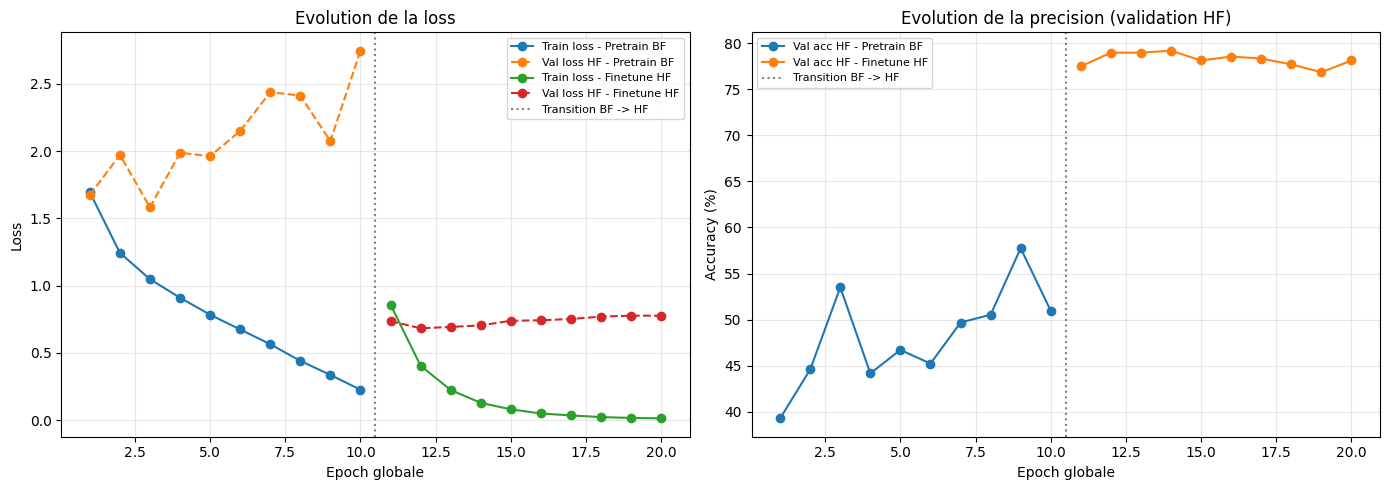
\includegraphics[width=0.96\linewidth,height=0.37\textheight,keepaspectratio]{figures/strategy1_transfer_learning_curves.png}\\[2pt]
    {\color{muted}\scriptsize Loss et pr\'{e}cision validation HF --- Strat\'{e}gie 1}
  \end{center}

  \vspace{0.08cm}
  \begin{columns}[T,onlytextwidth]
    \begin{column}{0.50\textwidth}
      \scriptsize
      \renewcommand{\arraystretch}{1.25}
      \arrayrulecolor{rule}
      \begin{tabular}{@{}lC{1.15cm}C{1.15cm}C{1.15cm}C{1.1cm}@{}}
        \toprule
        \color{primary}\textbf{M\'{e}thode} & \color{primary}\textbf{HF} & \color{primary}\textbf{BF} & \color{primary}\textbf{Mix} & \color{primary}\textbf{Co\^{u}t} \\
        \midrule
        \rowcolor{bfcolor!10}BL 2     & 59,07\% & 63,66\% & 61,36\% & 424k \\
        \rowcolor{accent!10}BL 3      & 75,90\% & 65,03\% & 70,47\% & 894k \\
        \rowcolor{success!18}\textbf{Strat.\ 1} & \textbf{78,84\%} & 57,65\% & 68,25\% & \textbf{400k} \\
        \bottomrule
      \end{tabular}
    \end{column}
    \begin{column}{0.47\textwidth}
      {\footnotesize\textbf{\color{primary}Protocole en deux phases}}
      \begin{itemize}\footnotesize\setlength\itemsep{2pt}
        \item \textbf{Pr\'{e}-entra\^{i}nement BF} (10 \'{e}poques, $lr=0.001$)
        \item \textbf{Fine-tuning HF} (10 \'{e}poques, $lr=0.0003$)
      \end{itemize}
      \scriptsize
      \textbf{\color{success}Points forts :} 78,84\% HF (meilleur score), $-$55\% de co\^{u}t vs BL3.\\
      \textbf{\color{danger}Limite :} Domain forgetting BF et l\'{e}ger overfitting en fin d'entra\^{i}nement.
    \end{column}
  \end{columns}
\end{frame}

% ============================================================
%  SECTION 7 : STRATÉGIE 2
% ============================================================
\begin{frame}{Strat\'{e}gie 2 --- Co-training par Batch avec Reweighting}
  \begin{center}
    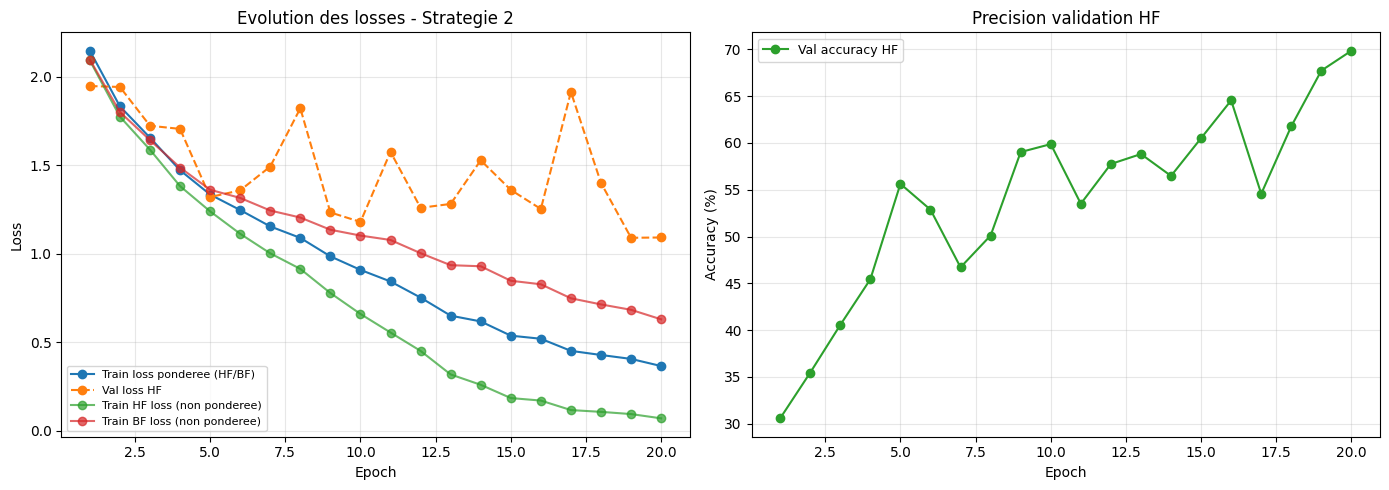
\includegraphics[width=0.96\linewidth,height=0.37\textheight,keepaspectratio]{figures/strategy2_cotraining_reweighting_curves.png}\\[2pt]
    {\color{muted}\scriptsize Losses et pr\'{e}cision HF --- Strat\'{e}gie 2}
  \end{center}

  \vspace{0.08cm}
  \begin{columns}[T,onlytextwidth]
    \begin{column}{0.50\textwidth}
      \scriptsize
      \renewcommand{\arraystretch}{1.25}
      \arrayrulecolor{rule}
      \begin{tabular}{@{}lC{1.15cm}C{1.15cm}C{1.15cm}C{1.1cm}@{}}
        \toprule
        \color{primary}\textbf{M\'{e}thode} & \color{primary}\textbf{HF} & \color{primary}\textbf{BF} & \color{primary}\textbf{Mix} & \color{primary}\textbf{Co\^{u}t} \\
        \midrule
        \rowcolor{accent!10}BL 3             & 75,90\% & 65,03\% & 70,47\% & 894k \\
        \rowcolor{success!10}Strat.\ 1        & 78,84\% & 57,65\% & 68,25\% & 400k \\
        \rowcolor{accent!12}\textbf{Strat.\ 2} & \textbf{70,12\%} & \textbf{61,90\%} & \textbf{66,01\%} & 486k \\
        \bottomrule
      \end{tabular}
    \end{column}
    \begin{column}{0.47\textwidth}
      {\footnotesize\textbf{\color{primary}M\'{e}canisme dual}}
      \begin{itemize}\footnotesize\setlength\itemsep{2pt}
        \item Batch mixte : \textbf{16 HF + 48 BF} (25\% HF)
        \item Pond\'{e}ration : $w_{HF}=2.0$, $w_{BF}=0.7$
        \item Entra\^{i}nement conjoint sur 20 \'{e}poques
      \end{itemize}
      \scriptsize
      \textbf{\color{success}Points forts :} robustesse BF (61,90\%) et gain de +13,9 pts HF vs BL1.\\
      \textbf{\color{danger}Limite :} performance HF inf\'{e}rieure \`{a} la Strat\'{e}gie 1 (70,12\% vs 78,84\%).
    \end{column}
  \end{columns}
\end{frame}

% ============================================================
%  SECTION 9 : BILAN
% ============================================================
\begin{frame}{Bilan comparatif complet}
\framesubtitle{Vue synoptique des 5 mod\`{e}les}
  \begin{columns}[T]
    \begin{column}{0.54\textwidth}
      \scriptsize
      \renewcommand{\arraystretch}{1.3}
      \arrayrulecolor{rule}
      \begin{tabular}{@{}lC{1.2cm}C{1.2cm}C{1.2cm}C{1.3cm}@{}}
        \toprule
        \color{primary}\textbf{Approche} & \color{primary}\textbf{HF} & \color{primary}\textbf{BF} & \color{primary}\textbf{Mix} & \color{primary}\textbf{Co\^{u}t} \\
        \midrule
        \rowcolor{hfcolor!8}BL 1 (HF)    & 56,20 & 35,16 & 45,68 & 470k \\
        \rowcolor{bfcolor!10}BL 2 (BF)   & 59,07 & 63,66 & 61,36 & 424k \\
        \rowcolor{accent!10}BL 3 (Mixte) & 75,90 & 65,03 & 70,47 & 894k \\
        \rowcolor{success!22}\textbf{Strat.\ 1} & \textbf{78,84} & 57,65 & 68,25 & \textbf{400k} \\
        \rowcolor{hfcolor!14}Strat.\ 2   & 70,12 & \textbf{61,90} & 66,01 & 486k \\
        \bottomrule
      \end{tabular}

      \medskip
      \begin{exampleblock}{\footnotesize R\'{e}sultat principal}
        \footnotesize \textbf{Strat\'{e}gie 1} d\'{e}passe BL3 sur HF\\
        (\textbf{78,84\% vs 75,90\%}) \`{a} \textbf{55\% du co\^{u}t} (400k vs 894k CA).
      \end{exampleblock}
    \end{column}
    \begin{column}{0.42\textwidth}
      \hspace*{0.15cm}
      \begin{tikzpicture}[x=0.044cm, y=0.78cm, font=\scriptsize]
        % cadre et grille
        \draw[rule, line width=0.4pt] (0, -0.55) rectangle (100, 4.65);
        \foreach \x in {0,20,40,60,80,100} {
          \draw[rule, dotted, line width=0.4pt] (\x, -0.55) -- (\x, 4.65);
          \node[anchor=north, text=muted, font=\tiny] at (\x, -0.65) {\x};
        }

        % labels à gauche
        \node[anchor=east, text=ink, font=\scriptsize] at (-4.5, 4.15) {Strat.1};
        \node[anchor=east, text=ink, font=\scriptsize] at (-4.5, 3.15) {BL3};
        \node[anchor=east, text=ink, font=\scriptsize] at (-4.5, 2.15) {BL2};
        \node[anchor=east, text=ink, font=\scriptsize] at (-4.5, 1.15) {BL1};
        \node[anchor=east, text=ink, font=\scriptsize] at (-4.5, 0.15) {Strat.2};

        % barres
        \fill[success] (0, 4.00) rectangle (78.84, 4.30);
        \fill[accent] (0, 3.00) rectangle (75.90, 3.30);
        \fill[bfcolor!70!black] (0, 2.00) rectangle (59.07, 2.30);
        \fill[bfcolor] (0, 1.00) rectangle (56.20, 1.30);
        \fill[hfcolor] (0, 0.00) rectangle (70.12, 0.30);

        \node[anchor=north, text=muted, font=\tiny] at (50, -0.95) {Pr\'{e}cision Test HF (\%)};
      \end{tikzpicture}
    \end{column}
  \end{columns}
\end{frame}

% ============================================================
%  PERSPECTIVES
% ============================================================
\begin{frame}{Perspectives et prochaines \'{e}tapes}
\framesubtitle{Optimisations cibl\'{e}es et axes de recherche}
  \begin{columns}[T]
    \begin{column}{0.47\textwidth}
      {\footnotesize\textbf{\color{primary}Am\'{e}liorations Strat\'{e}gie 1 (priorit\'{e} HF)}}
      \begin{itemize}\scriptsize\setlength\itemsep{1pt}
        \item \textbf{Epochs BF/HF} : tester 5/15, 8/12, 12/8 pour ajuster robustesse BF vs sp\'{e}cialisation HF
        \item \textbf{Learning rate par phase} : LR fine-tuning ni trop haut (oubli), ni trop bas (sous-adaptation)
        \item \textbf{Split HF train/val} : comparer 70/30, 80/20, 85/15 pour stabiliser la s\'{e}lection du meilleur mod\`{e}le
        \item \textbf{Fonction de co\^{u}t} : tester d'autres losses pour mieux g\'{e}rer bruit et classes difficiles
      \end{itemize}

      \medskip
      {\footnotesize\textbf{\color{primary}Am\'{e}liorations Strat\'{e}gie 2 (Co-training pond\'{e}r\'{e})}}
      \begin{itemize}\scriptsize\setlength\itemsep{1pt}
        \item \textbf{Ratio batch HF/BF} : le 16/48 (25\% HF) pilote directement le compromis HF/BF
        \item \textbf{Poids de loss} $w_{HF},w_{BF}$ : hyperparam\`{e}tres centraux de la m\'{e}thode
        \item \textbf{Fonction de loss alternative} : tester d'autres losses pour am\'{e}liorer la g\'{e}n\'{e}ralisation
        \item \textbf{Planning dynamique} : partir d'un poids HF mod\'{e}r\'{e}, puis l'augmenter progressivement (curriculum)
      \end{itemize}
    \end{column}
    \begin{column}{0.47\textwidth}
      {\footnotesize\textbf{\color{primary}Axes de recherche restants}}
      \begin{itemize}\footnotesize\setlength\itemsep{2pt}
       \item Tester d'autres strat\'{e}gies avanc\'{e}es (Noisy Student, etc.)
        \item Faire varier tous les param\`{e}tres et am\'{e}liorations possibles pour optimiser les strat\'{e}gies
        \item Tester d'autres jeux de donn\'{e}es
        \item Architecture backbone alternative (ResNet-34)        \item Variation du ratio HF/BF (5\%, 15\%, 20\%\ldots)
      \end{itemize}

      \medskip
      \begin{block}{\footnotesize Objectif de fin de projet}
        \footnotesize D\'{e}montrer rigoureusement qu'une approche multi-fid\'{e}lit\'{e} permet d'atteindre ou d\'{e}passer les performances d'un mod\`{e}le 100\% HF \`{a} \textbf{co\^{u}t d'annotation r\'{e}duit d'au moins 50\%}.
      \end{block}
    \end{column}
  \end{columns}
\end{frame}

% ============================================================
%  SLIDE DE CONCLUSION
% ============================================================
{
\setbeamertemplate{footline}{}
\setbeamertemplate{frametitle}{}
\begin{frame}[plain]
  \begin{tikzpicture}[overlay, remember picture]
    \shade[top color=primary, bottom color=primarydk]
      (current page.south west) rectangle (current page.north east);
    \fill[accent] (current page.south west) rectangle ([xshift=0.18cm]current page.north west);

    \fill[accent, opacity=0.10] ([xshift=-2.5cm, yshift=-1cm]current page.north east) circle (4.5cm);
    \fill[gold, opacity=0.12]   ([xshift=-1cm, yshift=-2cm]current page.north east) circle (2.2cm);

    \node[anchor=north west, text=accent, font=\footnotesize\bfseries]
      at ([xshift=0.95cm, yshift=-0.7cm]current page.north west)
      {CONCLUSION};
    \node[anchor=north west, text=white, font=\LARGE\bfseries]
      at ([xshift=0.95cm, yshift=-1.2cm]current page.north west)
      {Merci pour votre attention};
    \draw[accent, line width=0.8pt]
      ([xshift=0.95cm, yshift=-2.1cm]current page.north west) --
      ([xshift=2.5cm, yshift=-2.1cm]current page.north west);

    \node[anchor=north west, text=white!88, font=\small, text width=11cm]
      at ([xshift=0.95cm, yshift=-2.5cm]current page.north west)
      {La \textbf{\color{accent}Strat\'{e}gie 1 (Transfer Learning BF$\rightarrow$HF)} valide la faisabilit\'{e} de l'approche multi-fid\'{e}lit\'{e} : 78,84\% sur Test HF, d\'{e}passant la borne sup\'{e}rieure, \`{a} 55\% du co\^{u}t. };

    % KPI cards
    \node[anchor=south west] at ([xshift=0.95cm, yshift=1.6cm]current page.south west) {
      \begin{tikzpicture}
        \node[rounded corners=4pt, fill=success, text=white,
              minimum width=3cm, minimum height=1.3cm, align=center,
              drop shadow={shadow xshift=0pt, shadow yshift=-1pt, opacity=0.2}]
          {\Large\bfseries 78,84\%\\[1pt]\footnotesize Test HF};
      \end{tikzpicture}
    };
    \node[anchor=south west] at ([xshift=4.35cm, yshift=1.6cm]current page.south west) {
      \begin{tikzpicture}
        \node[rounded corners=4pt, fill=accent, text=white,
              minimum width=3cm, minimum height=1.3cm, align=center,
              drop shadow={shadow xshift=0pt, shadow yshift=-1pt, opacity=0.2}]
          {\Large\bfseries $-$55\% co\^{u}t\\[1pt]\footnotesize vs BL3};
      \end{tikzpicture}
    };
    \node[anchor=south west] at ([xshift=7.75cm, yshift=1.6cm]current page.south west) {
      \begin{tikzpicture}
        \node[rounded corners=4pt, fill=gold, text=primary,
              minimum width=3cm, minimum height=1.3cm, align=center,
              drop shadow={shadow xshift=0pt, shadow yshift=-1pt, opacity=0.2}]
          {\Large\bfseries 2 strat\'{e}gies\\[1pt]\footnotesize test\'{e}es};
      \end{tikzpicture}
    };
    \node[anchor=south west] at ([xshift=11.15cm, yshift=1.6cm]current page.south west) {
      \begin{tikzpicture}
        \node[rounded corners=4pt, fill=card, text=primary,
              minimum width=3cm, minimum height=1.3cm, align=center,
              drop shadow={shadow xshift=0pt, shadow yshift=-1pt, opacity=0.2}]
          {\Large\bfseries 5 mod\`{e}les\\[1pt]\footnotesize compar\'{e}s};
      \end{tikzpicture}
    };

    % Signature bas
    \node[anchor=south west, text=muted, font=\scriptsize]
      at ([xshift=0.95cm, yshift=0.7cm]current page.south west)
      {Ivann Vasic\ \textbullet\ Projet PF22\ \textbullet\ UTBM\ \textbullet\ Mars--Juin 2026};
  \end{tikzpicture}
\end{frame}
}

\end{document}
